\documentclass{article}

\usepackage{graphicx}
\usepackage{tikz}
\usepackage{tikzsymbols}
\usetikzlibrary{calc,patterns,shapes.geometric}
\pagestyle{empty}
\usepackage[margin=0pt]{geometry}
\geometry{papersize={14in,12in}}

\def\centerarc[#1](#2)(#3:#4:#5){\draw[#1] ($(#2)+({#5*cos(#3)},{#5*sin(#3)})$) arc (#3:#4:#5);}

\begin{document}
	\begin{figure}
		\centering
		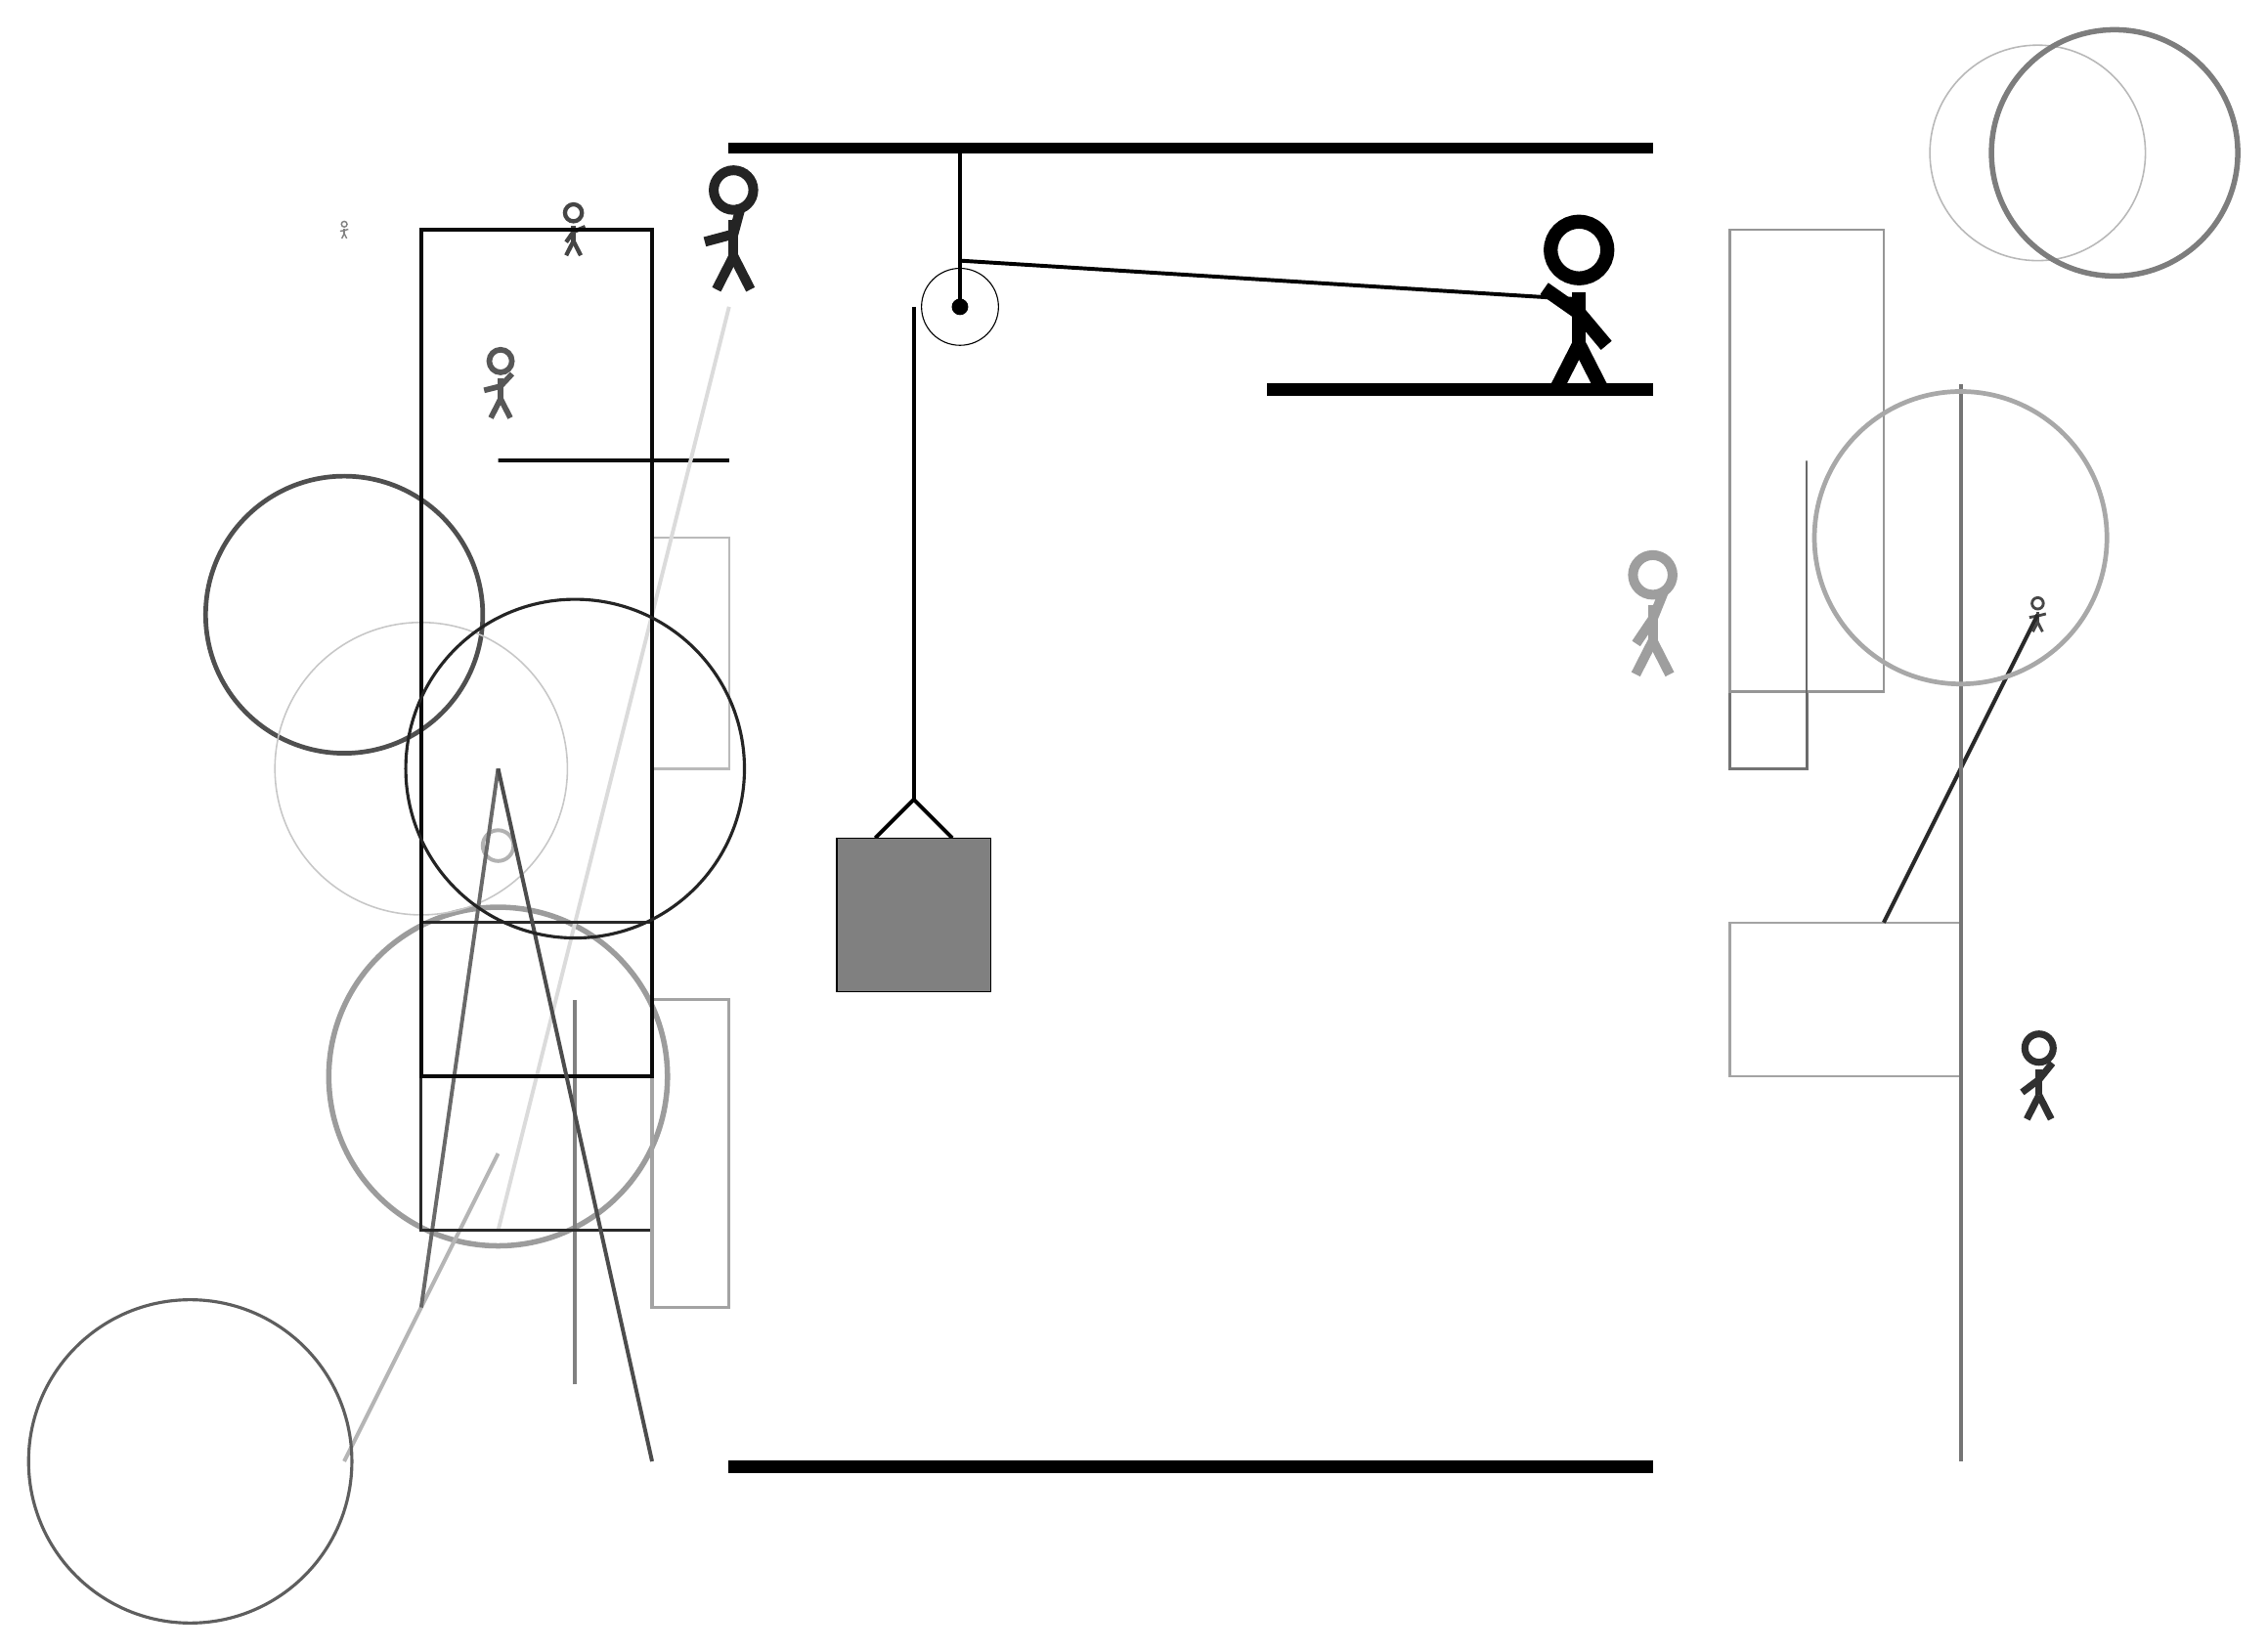
\begin{tikzpicture}
			%%%%% START %%%%%
			
			\draw[fill=black] (-2, 14) rectangle (10, 14.125);
			
			\draw (1, 12) circle (0.5);
			\draw[fill=black] (1, 12) circle (0.1);
			\draw[line width=0.5mm] (1, 14) -- (1, 12);
			
			\draw[line width=0.5mm](-0.1, 5.1) --  (0.4, 5.6) -- (0.9, 5.1);
			\draw[fill=black!50] (-0.6, 5.1) rectangle (1.4, 3.1);
			
			\draw[line width=0.5mm](0.4, 12) -- (0.4, 5.6);
			\centerarc[line width=0.5mm](1, 12)(90:180:0.6)
			\draw[line width=0.5mm](1, 12.6) -- (9, 12.1);
			
			\node at (9, 12) {\Strichmaxerl[10][-35][-50]};
			\draw[fill=black] (5, 11) rectangle (10, 10.85);
			
			\node[line width=0.6mm, color=black!72] at (15, 8) {\Strichmaxerl[2][10][14]};
			
			\draw[line width=0.4mm, color=black!55] (11, 7) rectangle (12, 6);
			\draw[line width=0.3mm, color=black!36] (11, 2) rectangle (14, 4);
			\draw [line width=0.7mm, color=black!39](-5, 2) circle (2.2);
			\node[line width=0.4mm, color=black!66] at (-5, 11) {\Strichmaxerl[4][14][47]};
			\draw[line width=0.5mm, color=black!84](13, 4) -- (15, 8);
			
			\draw[line width=0.5mm, color=black!29](-5, 1) -- (-7, -3);
			\draw [line width=0.5mm, color=black!30](-5, 5) circle (0.2);
			\draw[line width=0.5mm, color=black!90](-3, 7) -- (-3, 13);
			
			\draw [line width=0.2mm, color=black!28](15, 14) circle (1.4);
			
			\node[line width=0.3mm, color=black!86] at (-2, 13) {\Strichmaxerl[7][15][75]};
			\node[line width=0.6mm, color=black!81] at (15, 2) {\Strichmaxerl[5][37][51]};
			\draw[line width=0.5mm, color=black!95] (-2, 10) rectangle (-5, 10);
			
			\node[line width=0.6mm, color=black!49] at (-7, 13) {\Strichmaxerl[1][9][17]};
			\draw [line width=0.6mm, color=black!69](-7, 8) circle (1.8);
			\node[line width=0.5mm, color=black!73] at (-4, 13) {\Strichmaxerl[3][55][22]};
			\draw[line width=0.3mm, color=black!27] (-2, 6) rectangle (-3, 9);
			\draw[line width=0.5mm, color=black!54](14, -3) -- (14, 11);
			\draw [line width=0.2mm, color=black!22](-6, 6) circle (1.9);
			\draw[line width=0.5mm, color=black!59](-5, 6) -- (-6, -1);
			\draw[line width=0.5mm, color=black!14](-2, 12) -- (-5, 0);
			\draw[line width=0.3mm, color=black!41] (11, 7) rectangle (13, 13);
			\draw[line width=0.5mm, color=black!50](-4, -2) -- (-4, 3);
			\draw[line width=0.4mm, color=black!84] (-3, 0) rectangle (-6, 4);
			\draw[line width=0.4mm, color=black!36] (-2, 3) rectangle (-3, -1);
			\node[line width=0.7mm, color=black!38] at (10, 8) {\Strichmaxerl[7][56][68]};
			\draw[line width=0.5mm, color=black!96] (-3, 13) rectangle (-6, 2);
			\draw[line width=0.5mm, color=black!70](-5, 6) -- (-3, -3);
			\draw[line width=0.2mm, color=black!59] (12, 10) rectangle (12, 6);
			
			\draw [line width=0.4mm, color=black!86](-4, 6) circle (2.2);
			\draw [line width=0.4mm, color=black!63](-9, -3) circle (2.1);
			\draw [line width=0.6mm, color=black!34](14, 9) circle (1.9);
			\draw [line width=0.7mm, color=black!51](16, 14) circle (1.6);
			
			
			\draw[fill=black] (-2, -3) rectangle (10, -3.15);
			
			%%%%% END %%%%%
		\end{tikzpicture}
	\end{figure}	
\end{document}